\documentclass[tikz,border=7pt]{standalone}
\usetikzlibrary{calc}
\begin{document}
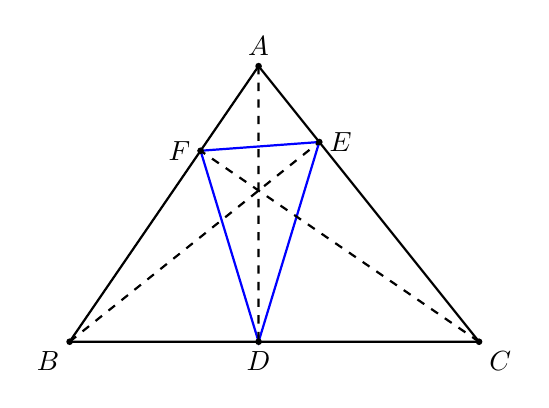
\begin{tikzpicture}[line width=.8pt]
\coordinate (A) at (0,3.5); \coordinate (B) at (-2.4,0); \coordinate (C) at (2.8,0);
\coordinate (D) at ($(B)!(A)!(C)$); \coordinate (E) at ($(C)!(B)!(A)$); \coordinate (F) at ($(A)!(C)!(B)$);
\draw (A)--(B)--(C)--cycle; \draw[blue,thick] (D)--(E)--(F)--cycle;
\draw[dashed] (A)--(D) (B)--(E) (C)--(F);
\foreach \p/\pos in {A/above,B/below left,C/below right,D/below,E/right,F/left} \fill (\p) circle (1.2pt) node[\pos] {$\p$};
\end{tikzpicture}
\end{document}
